% Pursuing Stacks (cotes 134-2 to 134-8): archive cote 134-4, site page 47 (PDF page 48), typescript page 135.
% typescript. Draft compared: ps3.tex:2384-2451.
% AI-transcribed by Claude Opus 5.5 (claude-opus-5-5, adaptive thinking, effort high), Message Batches API, batch ps2 (msgbatch_01NVwr1Yuo8qJf5rykeGBXPK), 2026-11-12; image review recorded in records/CHECK_DECISIONS_134_3_4.tsv.
\scanpage{134-4/47}
\mspage{135}
motopy interval in $M_2$ , namely $u(\hand{\delta}_o) \underset{h_2}{\hand{\sim}} u(\hand{\delta}_1)$ . If we assume moreover
that the intervals $\underline{I}$ in $\hand{\Sigma}^o_{h_1}$ are contractible, the previous condition is
equivalent to $u(I)$ being a contractible object of $M_2$ for any $\underline{I}$ in $\hand{\Sigma}^o_{h_1}$ .
T\over{h}{h}e case I am mainly thinking of of course is the one when $h_1$ can be des-%
cribed by a single generating weak homotopy interval, possibly even con-%
tractible, or even \inserted{by} a \inserted[typed]{(generating)} contractor. In the latter case, because of comm\unsure{\over[typed]{y}{u}}ta-%
tion of $u$ with finite products, $u(I)$ will be equally a contractor - and
contractible \inserted[typed]{for $h_2$} iff $u$ is a morphism of homotopy \over{\unsure{structures}}{structures}.

In the two precedent \inserted{paragraphs} \deleted{sections}, I forgot to mention the \xout{corresponding}
reduction of the corresponding compatibility conditions (of a functor $u$:
$M \hand{\longrightarrow} N$ , or of a saturated $W \hand{\subset} F\over{l}{\ell}(M)$) with a homotopy structure $h$, when
the latter is defined in terms of just a generating set $\hand{\Sigma}^o_h$ of weak homoto%
py intervals, possibly reduced to a single one, and moreover $u$ \uline{or} $W$
\margin{$\times$} \uline{are ``compatible with finite products''} . In the first case, it is enough
to check $u(\hand{\delta}_o)=u(\hand{\delta}_1)$ for any $\underline{I}$ in $\hand{\Sigma}^o_h$ \deleted{\unsure{x}} - and if $\underline{I}$ is contractible,
this amounts to demanding $u(\underline{I})$ is a final object of $N$. In the second case
it is enough \inserted{for strict compatibility, i.e. $W_h \subset W$} to check that \xout{\illegible{1}} for any $\underline{I}$ in $\hand{\Sigma}^o_h$ , $I \hand{\longrightarrow} e$ is in $W$. \unsure{(}\deleted{which is} \inserted{this condi-%
tion is also necessary, if any $\underline{I}$ in $\Sigma^o_h$ is contractible \deleted{and conversely, if the $I$'s are contractible}}
\xout{necessary and}\deleted{sufficient for \uline{strict} compatibility namely $W_h \subset W$}). Even if
$W$ is not \inserted[typed]{supposed} compatible with finite products namely $M \hand{\longrightarrow} W^{-1}M$ does not commute
with finite products, it is still sufficient \xout{that provided we assume}
\xout{even that strengthen the} for $W_h \hand{\subset} W$ that all $\underline{I}$'s in $\hand{\Sigma}^o_h$ be W-\uline{aspheric},
\hand{(}as stated in prop. (p.131)\hand{)}\hand{,} and this is necessary too, if the $\underline{I}$'s are
contractible.

\hand{4.4.}

5\over{5}{6}. This seemingly endless review of generalities on homotopy notions
is getting a little fastidious - and still I am not quite through yet
I feel. One main motivation for embarking on this review was one strong
impression which grew out of the reflections of now just one week ago
(\xout{\illegible{1}} paragraph 48), namely that the interesting``test functors'' from a
test category $A$ into a modelizer $(M,W)$ are those which factor through
the full subcategory $M_c$ of \uline{contractible} \uline{objects} of $M$. T\over{h}{h}e \inserted[typed]{presumable} extra condition\unsure{s}
% NOTE: the right edge of the scan cuts the end of the line "extra condition..." and of "weak homoto..." above
to put on \deleted{\xout{the}} \inserted[typed]{a} functor $A \hand{\longrightarrow} M_c$ to bor\over{r}{r}espond to an actual test functor $\hand{i}$
from $A$ to $M$ are strikingly weak, such as\hand{:} $i^{\hand{*}}(\hand{\Delta})$ should be \inserted[typed]{\xout{over}} \deleted{\xout{\illegible{1}}}aspheri\hand{c,}
\margin{\diagram{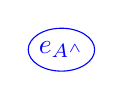
\begin{tikzpicture}[baseline=-.4ex,x=1em,y=1ex]\node[color=blue] at (0,0) {$e_{A^\wedge}$};\draw[color=blue,line width=.4pt] (0,0) ellipse (1.2 and 1.8);\end{tikzpicture}}} \inserted[typed]{over $\hand{e_{A^\wedge}}$} under the assumption we got a contractible generating homotopy interval
$\hand{\Delta}$ in $M$\hand{.} \xout{\illegible{1}} \over[typed]{i}{I}n any case, if $M^o_c$ is any full subcategory of $M_c$ which \xout{is}
gives rise (by taking intervals in $M^o_c$ ) to a \xout{generating} family of \inserted[typed]{homotopy} interva\hand{ls}
which \uline{generates} the homotopy structure $h_W$ on $M$ associated to $W$ , it should
\margin{47}
